\documentclass[14pt,a4paper]{extarticle}
\usepackage[utf8]{inputenc}
\usepackage[russian]{babel}
\DeclareUnicodeCharacter{00D7}{\(\times\)}

% геометрия страницы
\usepackage{geometry}
\geometry{top=2cm, right=1cm, bottom=2cm, left=2cm}

% математика, графики, объединение ячеек
\usepackage{amsmath}
\usepackage{graphicx}
\graphicspath{{images/}}
\usepackage{multirow}

% межстрочные отступы и шрифты
\usepackage{setspace}
\usepackage{pscyr}
%\renewcommand{\rmdefault}{ftm}

% подписи рисунков и таблиц по ГОСТу
\usepackage{caption}
\DeclareCaptionLabelFormat{figure}{Рисунок #2}
\DeclareCaptionLabelFormat{table}{Таблица #2}
\DeclareCaptionLabelSeparator{sep}{~---~}
\captionsetup{labelsep=sep,justification=centering,font=small}
\captionsetup[figure]{labelformat=figure}
\captionsetup[table]{labelformat=table}

% ссылки в pdf-файле
\usepackage{color}
\usepackage[colorlinks,linkcolor=black,urlcolor=black]{hyperref}
\renewcommand{\UrlFont}{\rm\small}

% центрированный столбец заданной ширины (в процентах от ширины страницы)
\usepackage{array}
\newcolumntype{C}[1]{>{\centering\arraybackslash}m{#1\textwidth}}
\renewcommand{\arraystretch}{1.2}

\begin{document}
  \begin{titlepage}
    \singlespacing
    \begin{center}
      Министерство образования и науки Российской Федерации \\
      Федеральное государственное бюджетное образовательное \\
      учреждение высшего профессионального образования \\
      <<Волгоградский государственный технический университет>> \\
      Факультет электроники и вычислительной техники \\
      Кафедра физики
    \end{center}

    \vspace{9em}

    \begin{center}
      \large Семестровая работа по дисциплине \\
      <<Радиоэлектроника>>
    \end{center}

    \vspace{5em}

    \begin{flushright}
      \begin{minipage}{.40\textwidth}
        Выполнили \\
        студенты группы Ф-469 \\
        Слоква В. И., \\
        Чечеткин И. А. \\

        \vspace{1em}

        Проверил профессор, \\
        доктор физ.-мат. наук \\
        Смоляр В. А.
      \end{minipage}
    \end{flushright}

    \vspace{\fill}

    \begin{center}
      Волгоград, \the\year
    \end{center}
  \end{titlepage}

  \setcounter{page}{2}
  \tableofcontents
  \newpage

  \section*{Параметры полупроводника}
  \addcontentsline{toc}{section}{Параметры полупроводника}

  \begin{table}[h!]
    \center
    \caption{Параметры полупроводника}
    \begin{tabular}{|l|C{.2}|} \hline
      \multicolumn{2}{|c|}{\bf Кремний (Si)} \\ \hline
      Эффективная масса электронов & \( 1,\!08 \cdot m_e \) \\
      Эффективная масса дырок & \( 0,\!56 \cdot m_e \) \\
      Энергия дна зоны проводимости,~эВ & \( 4,\!02 \) \\
      Энергия вершины валентной зоны,~эВ & \( 5,\!23 \) \\
      Ширина запрещенной зоны,~эВ & \( 1,\!21 \) \\ \hline
    \end{tabular}
  \end{table}

  \newpage

  \section{Концентрация электронов и дырок в собственном полупроводнике}

  Концентрация электронов в зоне проводимости равна:
  \begin{equation}
    n = 2\cdot\int\limits_{E_C}^\infty N(E) f(E, T) dE.
    \label{G1.9}
  \end{equation}

  Если уровень Ферми \( F \) лежит в запрещенной зоне энергий и удален от края
  зоны \( E_C \) хотя бы на \( 2kT \). Тогда в распределении Ферми-Дирака
  \eqref{G1.7}
  \begin{equation}
    f(E, T) = \frac{1}{1 + e^{\dfrac{E - F}{kT}}}
    \label{G1.7}
  \end{equation}
  единицей в знаменателе можно пренебречь и оно переходит в распределение
  Максвелла-Больцмана классической статистики (для кремния показаны на
  рис.~\ref{picF}). Это случай невырожденного полупроводника:
  \begin{equation}
    f(E, T) = e^{-\dfrac{E - F}{kT}}.
    \label{G1.8}
  \end{equation}

  \begin{figure}[h!]
    \center
    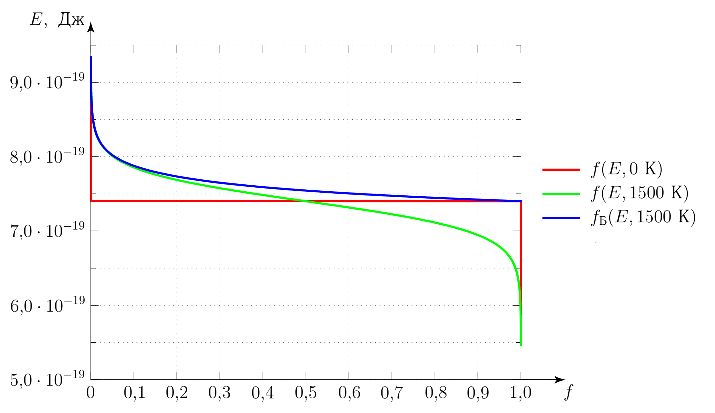
\includegraphics[width=.75\textwidth]{f(1500K)}\\
    \caption{Функции Ферми-Дирака \( f \) и Больцмана \( f_\emph{Б} \) для
      температуры 1500 К}
    \label{picF}
  \end{figure}

  Плотность состояний в зоне проводимости \( N(E) \) выражается формулой
  \begin{equation}
    N(E) = \frac{4\pi m_n^{3/2}\cdot\sqrt{2(E - E_C)}}{h^3},
    \label{G1.6}
  \end{equation}
  где \( m_n^{3/2} \)~-- эффективная масса электрона, \( E_C \)~-- энергия,
  соответствующая дну зоны проводимости.

  Если вместо \( (E - E_C) \) подставить \( (E_V - E) \), а вместо \( m_n \)~--
  эффективную массу дырки \( m_p \), то получим формулу плотности состояний в
  валентной зоне.

  Для кремния \( N(E) \) выглядит так, как показано на рисунке~\ref{picNE}.
  \begin{figure}[ht]
    \center
    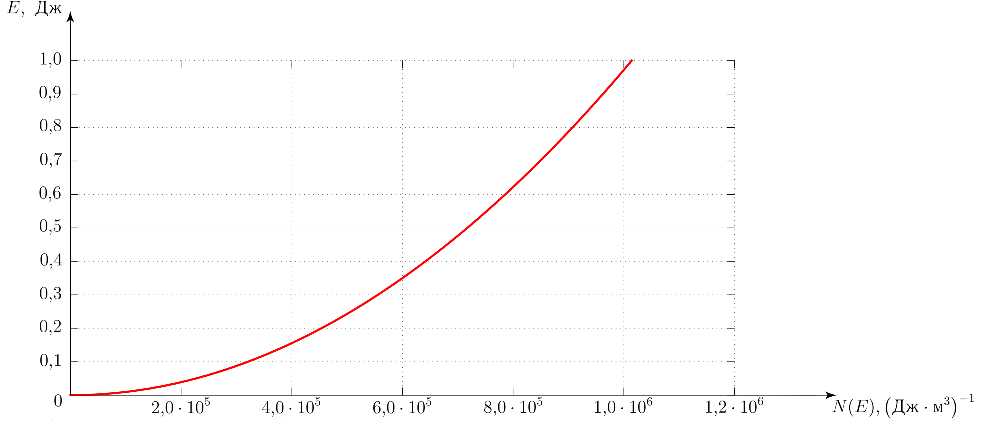
\includegraphics[width=.75\textwidth]{N(E)}
    \caption{Функция распределения плотности состояний в зоне проводимости
      \( N(E) \)}
    \label{picNE}
  \end{figure}

  \begin{figure}[b!]
    \center
    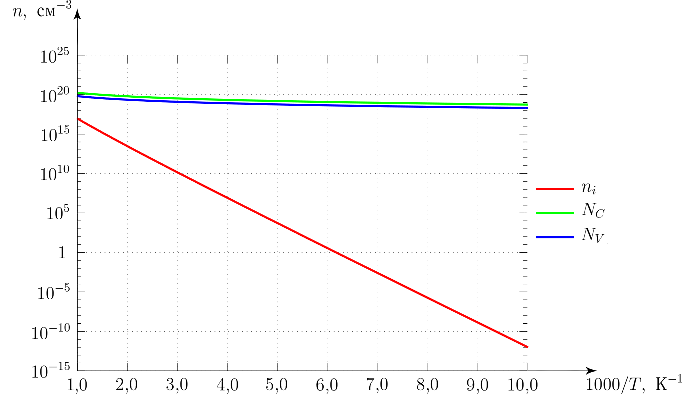
\includegraphics[width=.75\textwidth]{ni}
    \caption{Зависимость \( n_i(T) \), \( N_C(T) \), \( N_V(T) \)}
    \label{picNi}
  \end{figure}

  Подставив \eqref{G1.8} и \eqref{G1.6} в \eqref{G1.9}, получим:
  \begin{equation}
    n = N_C\cdot e^{-\dfrac{E_C - F}{kT}},
    \label{G1.10}
  \end{equation}
  где \( N_C \) -- эффективная плотность состояний в зоне проводимости:
  \[
    N_C = 2\cdot\left (\frac{2\pi m_n kT}{h^2} \right)^{3/2}.
  \]

  Концентрация дырок в валентной зоне:
  \begin{equation}
    p = N_V\cdot e^{-\dfrac{F - E_V}{kT}},
    \label{G1.13}
  \end{equation}
  где \( N_V \) -- эффективная плотность состояний в валентной зоне:
  \[
    N_V = 2\cdot\left (\frac{2\pi m_p kT}{h^2} \right)^{3/2}.
  \]

  Для расчета \( n \) и \( p \) по уравнениям \eqref{G1.10} и \eqref{G1.13}
  необходимо знать положение уровня Ферми \( F \). Однако произведение
  концентраций электронов и дырок для невырожденного полупроводника не зависит
  от уровня Ферми, хотя зависит от температуры:
  \begin{equation}
    n\cdot p = (n_i)^2 = N_C\cdot N_V\cdot e^{-\dfrac{E_g}{kT}}.
    \label{G1.14}
  \end{equation}

  Концентрацию собственных носителей заряда в зоне проводимости и в валентной
  зоне рассчитаем из формулы \eqref{G1.14}. Для кремния зависимость
  \( n_i(T) \), \( N_C(T) \), \( N_V(T) \) отображена на рисунке~\ref{picNi}.

  \newpage

  \section[Код программы]{Код программы на C (с использованием gnuplot)}
  {\small
  \begin{verbatim}
#include <stdio.h>
#include <stdlib.h>
#include <math.h>

const double e   = 1.6E-19;
const double m_e = 9.1E-31;
const double k   = 1.38E-23;
const double h   = 6.63E-34;
const double h2  = h * h;
const double h3  = h * h * h;

const float  m_p = 0.56 * m_e;
const float  m_n = 1.08 * m_e;
const float  E_c = 4.02;
const float  E_g = 1.21;
const float  E_v = E_c + E_g;
const float  F   = E_c + E_g / 2.0;

char elem_name[] = "Si";
char def_file[] = "data.txt";

double n_x(float m_x, float T)
{
  return 2.0 * pow(2.0 * M_PI * m_x * k * T / h2, 1.5) * 1E-6;
}

double fermi(double E, double T)
{
  return 1.0 / (1 + exp((E - F)*e / (k * T)));
}

double boltz(double E, double T)
{
  return exp(-(E - F)*e/(k * T));
}

double f(double m, double E)
{
  return 4.0 * M_PI * pow(m, 1.5) * sqrt(2.0 * (E - E_c)) / h3;
}

double n_e(float E)
{
  return 4.0 * M_PI * pow(m_n, 1.5) * sqrt(2.0 * (E - E_c*e) / h3);
}

int main(void)
{
  FILE *f, *p;
  const float T0 = 100.0f, T1 = 1000.0f, dt = 10.0f;
  float T, E;
  double N_c, N_v, n_i;

  f = fopen(def_file, "w");
  for (T = T0; T < T1; T += dt) {
    N_c = n_x(m_n, T);
    N_v = n_x(m_p, T);
    n_i = pow(N_c * N_v, 0.5f) * exp(-E_g * e / (2.0f * k * T));
    fprintf(f, "%.4E %.4E %.4E %.4E\n", 1000.0f / T, n_i, N_c, N_v);
  }
  fclose(f);

  p = popen("gnuplot -p", "w");
  fprintf(p,
    "set terminal pdfcairo enhanced color font 'Ubuntu, 10'\
       size 4.0in, 3.0in\n"
    "set border 3\n"
    "set grid\n"
    "set output 'n_i.pdf'\n"
    "set title '%s'\n"
    "set key outside right center spacing 1.3\n"
    "set logscale y\n"
    "set xtics 1.0\n"
    "set format x '%%.1f'\n"
    "set format y '10^{%%L}'\n"
    "set xlabel '1000/T, K^{-1}'\n"
    "set ylabel 'n, cm^{-3}'\n", elem_name);
  fprintf(p,
    "plot '%s' using 1:2 title ' n_i' with lines lc 1 lw 4 lt 1, "
    "'%s' using 1:3 title ' N_c' with lines lc 2 lw 4 lt 2, "
    "'%s' using 1:4 title ' N_v' with lines lc 3 lw 4 lt 5\n",
    def_file, def_file, def_file);
  pclose(p);

  f = fopen(def_file, "w");
  for (E = E_c - E_g / 2.0; E <= E_v + E_g / 2.0f; E += 1E-3) {
    fprintf(f, "%.4E %.4E %.4E %.4E %.4E %.4E %.4E %.4E\n",
      E*e, fermi(E, 0.001),
      fermi(E, 1500), boltz(E, 1500));
  }
  fclose(f);

  p = popen("gnuplot -p", "w");
  fprintf(p,
    "set terminal pdfcairo enhanced color font 'Ubuntu, 10'\n"
    "set border 3\n"
    "set grid\n"
    "set output 'f.pdf'\n"
    "set title '%s'\n"
    "set xrange [0:1]\n"
    "set xtics 0.1\n"
    "set format y '%%.1t×10^{%%T}'\n"
    "set key outside right center spacing 1.3\n"
    "set xlabel 'f'\n"
    "set ylabel 'E, J'\n", elem_name
 );
  fprintf(p,
    "plot '%s' using 2:1 title 'Fermi, T = 0 K'\
      with lines lc 1 lw 4 lt 1, "
    "'%s' using 3:1 title 'Fermi, T = 1500 K'\
      with lines lc 2 lw 4 lt 1, "
    "'%s' using 4:1 title 'Boltzmann, T = 1500 K'\
      with lines lc 3 lw 4 lt 1\n",
    def_file, def_file, def_file);

  pclose(p);

  f = fopen(def_file, "w");
  for  (E = 0.0f; E < 1.0f; E += 1E-3) {
    fprintf (f, "%.4E %.4E\n", E, n_e (E));
  }
  fclose (f);

  p = popen("gnuplot -p", "w");
  fprintf(p,
    "set terminal pdfcairo enhanced color font 'Ubuntu, 10'\n"
    "set border 3\n"
    "set grid\n"
    "set output 'N_E.pdf'\n"
    "set title '%s'\n"
    "set format x '%%.1t×10^{%%T}'\n"
    "set format y '%%.2f'\n"
    "set xrange [0:*]\n"
    "set xlabel 'N(E)'\n"
    "set ylabel 'E, J'\n", elem_name
  );
  fprintf(p,
    "plot '%s' using 2:1 notitle with lines lc 1 lw 4 lt 1\n", def_file);
  pclose(p);
  return EXIT_SUCCESS;
}
  \end{verbatim}
  }

  \newpage

  \begin{thebibliography}{9}
    \addcontentsline{toc}{section}{Список литературы}
    \bibitem{1} Гуртов,~В.~А. Твердотельная электроника: Учеб. пособие~/
      В.~А.~Гуртов.~-- М., 2005.~-- 492~с.
    \bibitem{2} NSM Archive~-- Physical Properties of Semiconductors \\
      \url{http://www.matprop.ru/semicond}
  \end{thebibliography}

\end{document}